% write your main thesis in logical individual chapters
% for better organization use a separate folder for images
\graphicspath{{img/}}








%==============================
\chapter{Pregled metod medplaformnega razvoja}
\label{chap:overview}

Predno postavimo omejitve razvoja naše aplikacije, si poglejmo različne metode medplatformnega razvoja in v katerih primerih jih je pametno uporabiti. Kot je pričakovati, jih je kar nekaj. Razdelili jih bomo v skupine celovitih, delnih in deljenih metod.

%-----
\section{Celovit}

Celovita metoda za razvoj uporablja ogrodje, s pomočjo katerega aplikacijo pripravimo za različne platforme. Velika večina tako napisane izvorne kode je uporabljena na vseh destinacijskih platformah, za kar poskrbi ogrodje. Rezultat te metode je domorodna aplikacija, ki jo je možno objaviti v trgovinah posameznih platform in pri tem ne kršijo (ponavadi) strogih pravil.

\subsection{Qt}

Qt\footnote{\href{http://qt-project.org}{http://qt-project.org}} je ogrodje za grafično programiranje za več platform s pomočjo jezika C++ in QML\footnote{Qt Meta Language ali Qt Modeling Language, vir \href{http://en.wikipedia.org/wiki/QML}{Wikipedia}}. Omogoča nam sočasni razvoj za platforme OSX, Linux, Windows, Android in iOS. Podpira tudi uporabo HTML5\footnote{\href{http://en.wikipedia.org/wiki/HTML5}{http://en.wikipedia.org/wiki/HTML5}} namesto QML, kar pomeni, da spletni razvijalci lahko uporabijo že obstoječe znanje in učenje novega jezika ni potrebno.

Qt projekt je povsem odprtokoden in dovoljuje uporabo v skladu z licencama GPL v3\footnote{\href{http://www.gnu.org/copyleft/gpl.html}{http://www.gnu.org/copyleft/gpl.html}} in LGPL v2.1\footnote{\href{https://www.gnu.org/licenses/old-licenses/lgpl-2.1.html}{https://www.gnu.org/licenses/old-licenses/lgpl-2.1.html}}, a če želite orodje uporabiti za razvoj mobilne aplikacije, boste morali za to odšteti 149\$ mesečno.

Projekt so vrsto let uspešno razvijali v podjetju Nokia, kjer so ga uporabili kot glavno orodje za razvoj aplikacij na platformi Symbian. Ko je pred časom Microsoft kupil podjetje Nokia, je projekt prevzela novonastala organizacija Qt Project, ki projekt vodi še danes.

Qt je še posebej privlačen zaradi podpore namiznih platform kot so Windows, Mac OSX in Linux. Odlikuje ga tudi zagreta skupnost razvijalcev.

Glavne slabosti Qt so neskladnost z izgledom ostalih aplikacij na mobilnih platformah, plačljiva licenca za razvoj mobilnih aplikacij ter končna velikost samih programov.

\subsection{Xamarin}

Xamarin\footnote{\href{https://xamarin.com}{https://xamarin.com}} je ogrodje za sočasen razvoj aplikacij za platforme iOS, Android, Mac in Windows v jeziku C\#. Izjaha iz projekta Mono\footnote{\href{http://www.mono-project.com}{http://www.mono-project.com}}, ki omogoča uporabo ogrodja .NET na različnih platformah.

Ogrodje omogoča razvoj aplikacij, katerih izgled je skladen z ostalimi aplikacijami na izbrani platformi. Kot primer si lahko ogledamo aplikacijo za poslušanje glasbe Rdio\footnote{\href{https://www.rdio.com}{https://www.rdio.com}}, ki je na voljo za iOS, Android in Windows Phone.

Ogrodje odlikuje integrirano razvojno okolje (IDE), ki razvoj aplikacij znatno olajša. Omogoča testiranje tako v emulatorju/simulatorju kot na samih napravah.

Glavna slabost ogrodja Xamarin je cena, saj se paketi začnejo šele pri 299\$/mesec za vsakega razvijalca in vsako platformo posebej. Za majhno ekipo je lahko taka začetna cena enostavno previsoka. Vprašljiva je tudi hitrost dodajanja funckionalnosti posameznih platform, ko se te nadgradijo, določen riziko predstavlja tudi muhavost posameznih platform pri omejitvah uporabe tega ogrodja, sploh če nadgradnja povzroči nedelovanje takih aplikacij.

\subsection{Adobe Air}

Adobe Air je brezplačno ogrodje, ki omogoča zagon iste aplikacije na platformah iOS, Android, Mac, Windows in Linux. Čeprav za razvoj namiznih aplikacij omogoča uporabo HTML in Javascript, je za razvoj mobilnih aplikacij omejen na uporabo jezika ActionScript. V času pisanja diplomske naloge ogrodje ne omogoča zagon na platformi Windows Phone, vendar so razvijalci podporo že napovedali.

Izbor orodja je še posebej uporaben za razvoj iger, kjer se razvijalcem ni treba prav preveč prilagajati domorodnim aplikacijam.

Kot glavno slabost ogrodja Adobe Air bi navedel upadanje zanimanja za orodje Flash. Špekuliramo lahko tudi o planih podjetja Adobe, saj so pred kratkim kupili podjetje Nitobi, ki je avtor ogrodja PhoneGap (katerega si ga bomo ogledali v nadaljevanju). Uporaba tudi ni primerna za razvoj klasičnih mobilinih aplikacij, saj je prilagajanje domorodnim aplikacijam precej zahtevno, še posebej kadar na platformi pride do posodobitve izgleda.

%-----
\section{Hibriden}

Hibridna metoda za razvoj aplikacij uporablja spletne tehnologije v sožitju z kodo za posamezno platformo (t.i. premostitvena tehnika), ki omogoča dostop do glavnih funkcij naprav (kot so kamera, pospeškomer in podobno). Tako kot pri celovitih metodah, je tudi tu rezultat domorodna aplikacija, ki jo je možno objaviti v trgovinah posameznih platform.

\subsection{Apache Cordova / PhoneGap}

Ogrodje Apache Cordova\footnote{\href{http://cordova.apache.org}{http://cordova.apache.org}} je odprtokodni projekt, ki omogoča objavo spletnih aplikacij kot domorodne. V času pisanja diplomske naloge ogrodje podpira iOS, Android, Windows Phone, Blackberry, Palm WebOS, Bada in Symbian. Na vseh omenjenih platformah nam ogrodje Apache Cordova omogoča dostop do funkcij naprave, ko so naprimer kamera in pospeškomer.

Projekt PhoneGap\footnote{\href{http://phonegap.com}{http://phonegap.com}} je dejansko samo ena od distribucij projekta Apache Cordova, ki poleg vseh obstoječih funkcionalnosti ponuja tudi razne storitve na katerih delajo v podjetju Adobe.

Za razvoj aplikacij razvijalci lahko uporabljajo spletne tehnologije HTML, CSS in JavaScript. S pomočjo ogrodij jQuery Mobile in Sencha Touch je možno izdelati aplikacije, katerih izgled je zelo lep približek ostalim aplikacijam na izbrani platformi. Če naletimo na funkcijo naprave, do katere nimamo dostopa, ali ugotovimo da je JavaScript za določene naloge premalo učinkovit, lahko preprosto spišemo lasten vtičnik, ki služi kot most med kodo napisano v jeziku JavaScript in domorodno kodo.

Glavna prednost ogrodja Apache Cordova in predvsem distribucije PhoneGap je izredno nezahtevnost ogrodja. Priporoča se predvsem za izdelavo prototipnih aplikacij, saj nam omogoča hiter razvoj in iteracijo.

Glavna slabost tega pristopa tiči v performanci in odzivnosti aplikacije, saj ta za prikazovanje izkorišča vgrajeno spletno okno. Trenutno je težko izdelati aplikacije, ki so grafično zahtevnejše, kar pomeni še toliko bolj pereč problem na napravah s slabšimi karakteristikami. Da se aplikacija po izgledu nebi ločila od domorodnih aplikacij je potrebno vložiti kar nekaj dela, na koncu pa bo izurjen uporabnik najbrž vseeno opazil, da je aplikacija malce drugačna. Problem predstavlja tudi zamik podpore novim stilom grafičnih elementov, tako kot se je to zgodilo pri prehodu iz iOS6 na iOS7.

\subsection{Appcelerator Titanium}

Ogrodje Titanium nam omogoča izdelavo aplikacij za več platform hkrati s pomočjo JavaScript okolja, ki služi kot abstrakcijska plast med našo aplikacijo in domorodno kodo. Aplikacijo gradimo s pomočjo jezika JavaScript, ki se med uporabo aplikacije izvaja s pomočjo pogona V8 (Android), JavaScriptCore (iOS) ali vgrajenega JavaScript okolja (če aplikacijo poganjamo v brskalniku). Za pravilen vizualen izgled skrbijo namestniški elementi, ki uporabljajo domorodne grafične elemente, kar pomeni da vizualno aplikacije ne ločimo od ostalih domorodnih aplikacij. V času pisanja diplomske naloge ogrodje podpira iOS, Android, Blackberry, Tizen in spletne aplikacije.

Glavna prednost ogrodja Titanium ni t.i. način piši enkrat, uporabljaj povosd; njegova prednost je da lahko celotno aplikacijo izdelamo v enem jeziku - JavaScript-u. Le redko se bomo srečali z domorodno kodo, saj ogrodje nudi široko paleto knjižnic.

Glavna slabost ogrodja je počasno dodajanje novih platform zaradi obsežnosti dela, ki ga tak podvig zahteva. Določene knjižnice za delo z domorodnimi elementi tudi niso najbolj performančne, manjka pa tudi napovedana podpora platformi Windows Phone.

%-----
\section{Deljen}

Deljena metoda za razvoj aplikacij omogoča uporabo dela aplikacijske kode na vseh platformah za katere razvijamo. To lahko naredimo s pomočjo vgradnega skriptnega jezika (Lua), s pomočjo prevajanja iz izbranega programskega jezika v domorodnega (Haxe, XMLVM, emscripten) ali pa z uporabo programskega jezika C++ in programskimi ovoji, s katerimi pripravimo knjižnico za vgradnjo v druge platforme.

\subsection{Lua}

Lua\footnote{\href{http://www.lua.org}{http://www.lua.org}} je preprost vgradni skriptni jezik, ki ga odlikuje hitrost izvajanja in procesorska nezahtevnost. Vgradimo ga lahko v platforme Android, iOS, Symbian in Windows Phone, z nekaj potrpljenja pa lahko isto kodo zaženemo tudi v spletni aplikaciji.

Čeprav je jezik Lua preprost za uporabo, se izkaže da za kompleksnejše knjižnice ni primeren. Manjka tudi Unicode podpora in boljša podpora rokovanju z napakami.

// TODO Standardna knjižnica?, več razlage o načinu uporabe.

\subsection{Haxe}

Haxe\footnote{\href{http://haxe.org}{http://haxe.org}} zase pravi, da je večplatformski programski jezik. Razvijalec lahko svojo aplikacijo napiše v jeziku Haxe, nato pa jo s pomočjo prevajalnika prevede v JavaScript, C++, C\# ali Javo.

Pri prevajanju aplikacije v ciljni jezik Haxe povzroči ne tako zanemarljivo napihnjenje kode, saj v želji dobesednega prevoda na vsako od ciljnih platform prenese svoje delovanje plus kodo, ki smo jo napisala za našo aplikacijo.

// TODO več razlage o načinu uporabe, prednostih in slabostih

\subsection{XMLVM}

XMLVM\footnote{\href{http://xmlvm.org}{http://xmlvm.org}} spada v isti razred kot Haxe - tako imenovanih prevajalcev iz enega jezika v drugega (ang. cross-compilers), a se XMLVM tega loti na drugačen način. Medtem ko Haxe prevaja na nivoju izvorne kode, XMLVM to počne na nivoju zlogovne kode (ang. byte code). Izvorna koda je lahko napisana za navidezne stroje (ang. virtual machine) JVM, .NET CLI ali Ruby YARV, medtem ko je rezultat delujoč program za JVM, .NET CLI, Javascript, Pyhton, Objective-C in C++.

\begin{figure}
 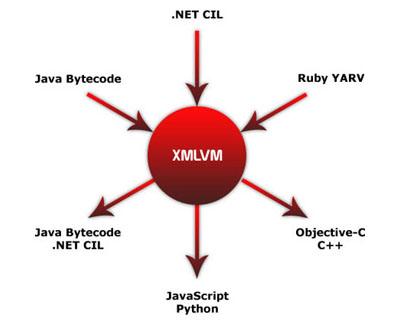
\includegraphics[scale=0.5]{xmlvm}
 \caption{XMLVM}
 \label{fig:xmlvm}
\end{figure}

Projekt izgleda zelo ambiciozen, a vse kaže da je šlo le za akademsko raziskavo, saj je v času pisanja diplome minilo že več ko leto dni odkar se je izvorna koda posodobila. Kljub temu se mi je projekt zdel zanimiv in ga je bilo vredno izpostaviti.

\subsection{C++ in emscripten}

V kolikor nobena od naštetih možnosti ne zadošča našim potrebam, želeli pa bi vseeno imeti deljeno knjižnico, obstaja še ena možnost: uporaba jezika C++\footnote{\href{http://www.cplusplus.com}{http://www.cplusplus.com}} in projekta emscripten\footnote{\href{http://emscripten.org}{http://emscripten.org}}.

C++ je eden izmed najbolj razširjenih programksih jezikov. V času pisanja diplomske naloge zaseda četrto mesto na lestvici najbolj popularnih jezikov \ref{fig:tiobe-index}, pred njim so samo C, Java in Objecitve-C. Uporablja se ga v raznolikih projektih, od prevajalnikov, strežnikov, do video igric.

\begin{figure}
 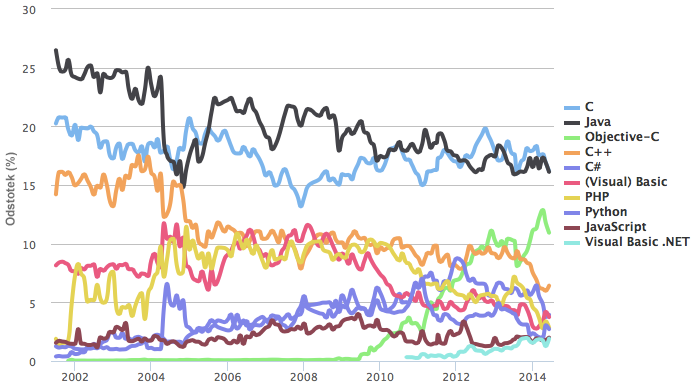
\includegraphics[width=\linewidth]{tiobe-index}
 \caption{Tiobe programming comunity index \protect\href{http://www.tiobe.com/index.php/content/paperinfo/tpci/index.html}{http://www.tiobe.com/index.php/content/paperinfo/tpci/index.html}}
 \label{fig:tiobe-index}
\end{figure}

Emscripten je projekt Mozilinih laboratorijev ki omogoča prevajanje iz LLVM\footnote{Low Level Virtual Machine} zlogovne kode v skriptni jezik JavaScript. LLVM si lahko predstavljamo kot vmesni sloj med izvorno (C, C++, Objective-C, Java, C\#) in strojno kodo, ki skrbi poskrbi za visoko optimizacijo vmesne kode, to pa lahko potem prevedemo v ustrezen nabor ukazov za posamezne procesorje (ARM, x86 itd.). Emscripten tako predstavlja zadnjo fazo prevajalnika, le da vmesne kode iz LLVM ne prevede v ukaze specifičnega procesorja, ampak prevede nazaj v jezik JavaScript. To seveda pomeni, da lahko prevedemo skoraj vsak program (z določenimi omejitvami) v JavaScript in ga zaženemo v brskalniku. Celo grafično zahtevne aplikacije niso problematične, saj emscripten za prevod v JavaScript uporablja asm.js\footnote{\href{http://asmjs.org}{http://asmjs.org}}, kar je podmnožica jezika JavaScript, ki jo JavaScript pogoni znajo izredno dobro optimizirati.

\begin{figure}
 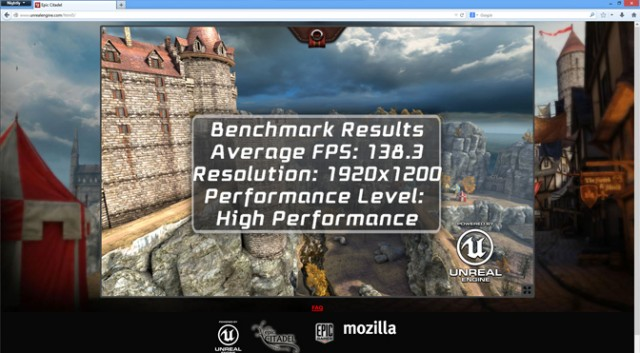
\includegraphics[width=\linewidth]{emscripten-epic-citadel}
 \caption{Skupina Mozilinih inžinirjev je grafično ogrodje Unreal v štirih dneh posodobilo do te mere, da je lahko s pomočjo orodja emscripten grafično zahtevna aplikacija brezhibno delovala v brskalniku.}
 \label{fig:epic-citadel}
\end{figure}

%==============================
\chapter{Razvoj knjižnice}
\label{chap:development}

%-----
\section{Omejitve}

Predno se lotimo izbora primerne metode postavimo nekaj omejitev:

\begin{enumerate}
  \item Delovati mora na platformah iOS, Android, Windows Phone in spletu.
  \item Zagotavljati grafično skladnost z ostalimi domorodnimi aplikacijami.
  \item Imeti dovolj razgibano razvijalsko skupnost, da bomo lahko našli odgovore na nastale probleme.
  \item Mora biti odporna na spremembe pri nadgradnjah platforme.
\end{enumerate}

Izbrano rešitev želimo prikazati na primeru aplikacije, ki prikazuje ponavaljajoče si dogodke s pomočjo standarda RFC 5545\footnote{\href{http://tools.ietf.org/html/rfc5545}{http://tools.ietf.org/html/rfc5545}}. Zaradi poenostavitve se bomo osredotočili zgolj na del RRULE{\footnote{\href{http://tools.ietf.org/html/rfc5545\#section-3.3.10}{http://tools.ietf.org/html/rfc5545\#section-3.3.10}}}, ki definira pravila za ponavljanje dogodka.

Poglejmo si primer kompleksnega pravila za ponavljanje dogodka:

\begin{lstlisting}
FREQ=YEARLY;INTERVAL=2;BYMONTH=1;BYDAY=SU;BYHOUR=8,9;BYMINUTE=30
\end{lstlisting}

Če prevedemo to v človeku prijazno obliko, bi to pomenilo ``vsako nedeljo v januarju ob 8:30 zjutraj in 9:30 zjutraj, vsako drugo leto''.

Ponavljajoč dogodek bo aplikacija prikazala v preprostem seznamu, ki bo prilagojen za vsako od izbranih platform.

// slika iOS seznama z vsemi podatki ki bodo prikazani

%-----
\section{Izbor primerne metode}

Izbor primerne metode lahko začnemo z pregledom popularnih vprašanj na spletni strani Stackoverflow. Ta nam da lahko hiter pregled v aktivnost posameznih razvijalskih skupnosti.

\begin{figure}
 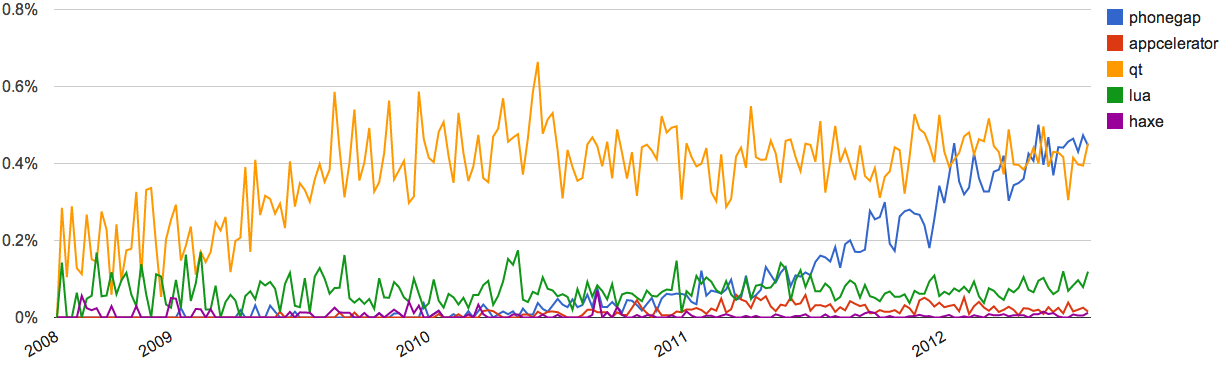
\includegraphics[width=\linewidth]{stackoverflow-trends}
 \caption{Prikaz trendov za nekaj od predlaganih rešitev na spletni strani Stackoverflow, kjer razvijalci iščejo rešitve problemov na katere so naleteli.}
 \label{fig:stackoverflow-trends}
\end{figure}

Grafično prilagajanje domorodnim aplikacijam.

Xamarin -> slabost cena
PhoneGap -> neskladnost
Appcelerator -> ni zastonj

%-----
\section{C++}

%-----
\section{Emscripten}

%==============================
\chapter{Vključitev knjižnice v različne platforme}
\label{chap:cross-platform}

%-----
\section{iOS}

%-----
\section{Android}

%-----
\section{Windows Phone}

%-----
\section{Spletna aplikacija}
